\documentclass[12pt]{article}
\usepackage[scaled]{helvet}
\renewcommand\familydefault{\sfdefault} 
\usepackage[T1]{fontenc}

\usepackage[english]{babel}
\usepackage[utf8]{inputenc}
\usepackage{amsmath}
\usepackage{bm}
\usepackage{parskip}
\usepackage{hyperref}
\usepackage{graphicx}
\usepackage{listings}
\usepackage{xcolor}

\definecolor{Brown}{cmyk}{0,0.81,1,0.60}
\definecolor{OliveGreen}{cmyk}{0.64,0,0.95,0.40}
\definecolor{CadetBlue}{cmyk}{0.62,0.57,0.23,0}
\definecolor{lightlightgray}{gray}{0.9}

\lstset { %
    language=C++,
    %backgroundcolor=\color{black!5}, % set backgroundcolor
    %basicstyle=\footnotesize,% basic font setting
	basicstyle=\ttfamily,                   % Code font, Examples: \footnotesize, \ttfamily
	keywordstyle=\color{OliveGreen},        % Keywords font ('*' = uppercase)
	commentstyle=\color{gray},              % Comments font
	backgroundcolor=\color{lightlightgray},
	tabsize=4,
	frame=single,
}

\title{\textbf{Practical 4: Mass-Spring Systems, part 1 }}
\author{Babis Koniaris}
\date{}

\begin{document}
\maketitle

\begin{center}
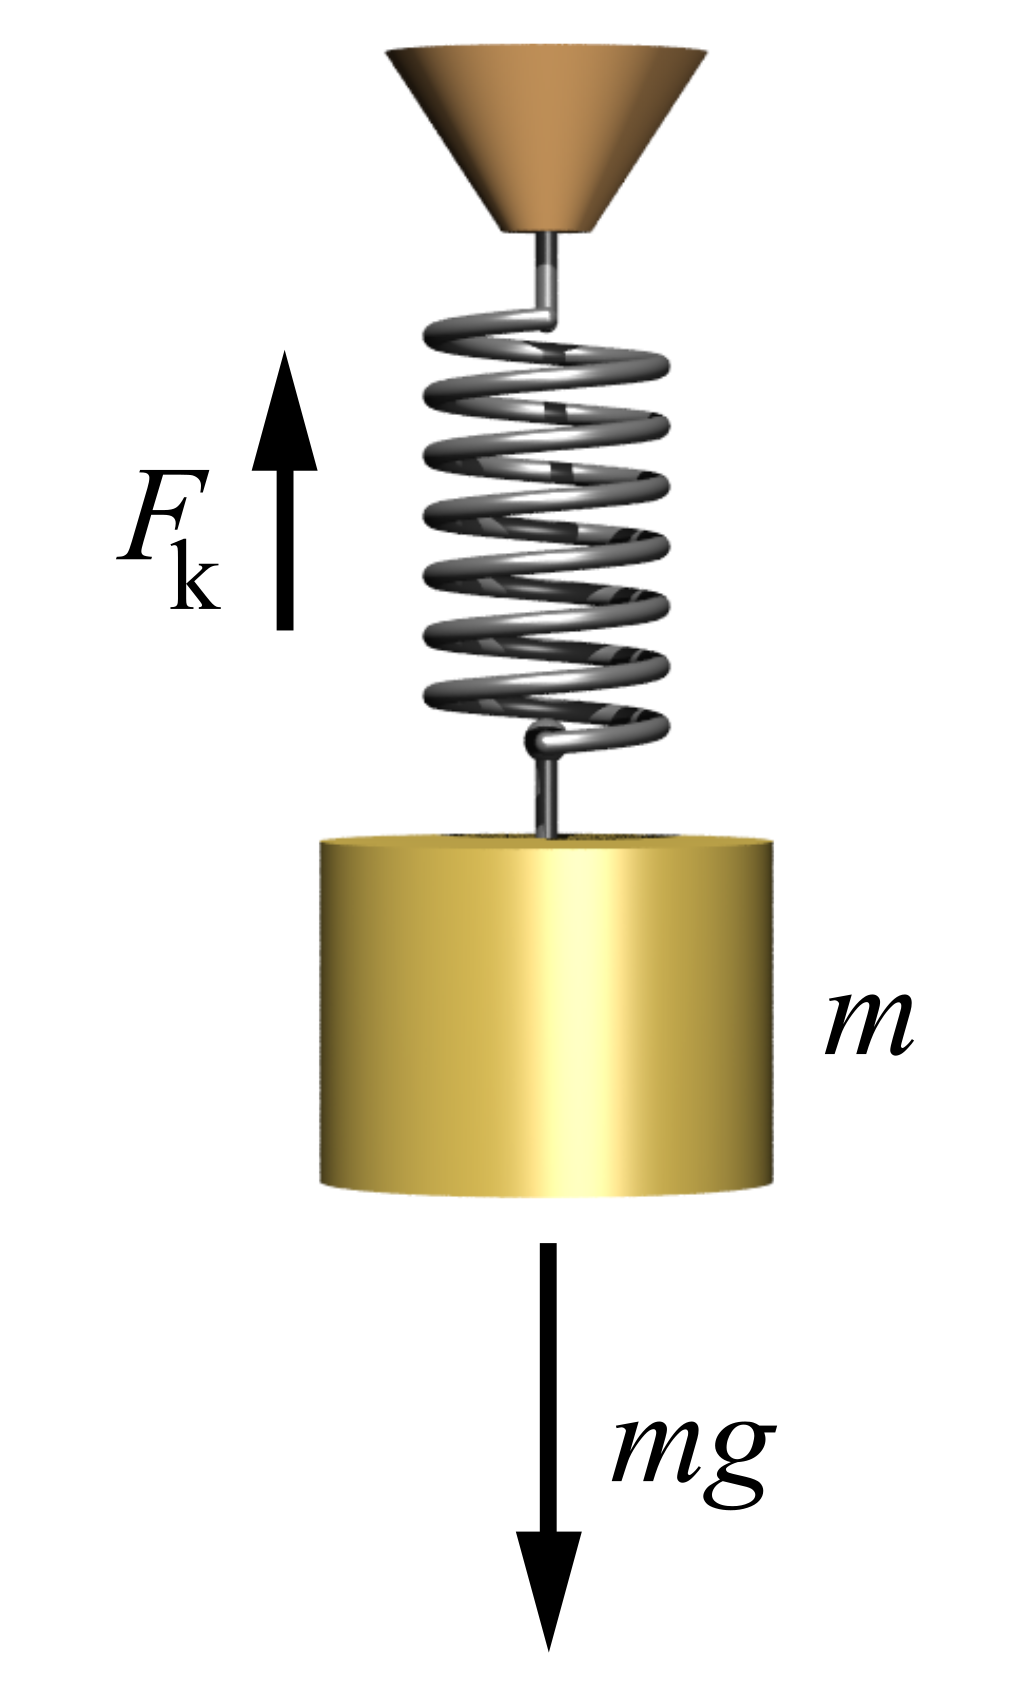
\includegraphics[width=0.6\textwidth]{p4-teaser.png}
\end{center}
\pagebreak

\section*{Introduction}

The goal of this practical are to:

\begin{itemize}
\item Revise our architecture to support the implementation of mass-spring systems
\item Develop a practical understanding of constrained particle systems
\item Implement 1D mass-spring system simulations
\end{itemize}

\section*{Architecture changes}

To assist with the requirements of constrained particle systems, a slightly modified project is provided for you: ``03\_constraints\_framework''. There are only a few key differences compared to the previous framework:

\begin{itemize}
\item The Particle class (declared in PhysicsObject.h) now stores accumulated (per update iteration) forces and impulses. During simulation, you first clear the forces and impulses (Particle::ClearForcesImpulses), the process all your particles and apply and required forces or impulses (Particle::ApplyForce and Particle::ApplyImpulse), and finally, at the integration step you will get the accumulated forces and impulses in order to compute acceleration, new velocity and new position for each particle.
\item The forces are now more explicit, and we provide a function for each. You can see the function declarations in Force.h. Only the gravity implementation has been implemented for you, so you can implement the rest using the formulas in the lecture materials. When you calculate a force, you should call .ApplyForce(...) on the particle, to add the force into its list of forces. You can see that Hooke force is a bit special, as it applies (opposing) force to two particles. You will notice that the particles are passed in by reference, so that we can modify them (their accumulated force, via ApplyForce).
\end{itemize}

You can copy over relevant code from your previous project, so that your timestep and integration functionality is already implemented. The part that we will be changing in these two practicals is the application and evaluation of forces and impulses.

\section*{Tasks}

\subsection*{Task 1: Port integration and timestep to new project}

Before you start working on mass-spring systems, make sure that this new project includes integration (one method will suffice) and timestep from the last project, so that you have a single particle bouncing around a cubic room, or just off the ground. While the code for integration and timestep should be mostly identical (and copied over), the part that changes is how do you get a vec3 for the force, and a vec3 for the impulse. The previous section describes the changes that need to be done to achieve that, and can be summarised as:

\begin{itemize}
\item At the beginning of a particle's simulation step, call particle.ClearForcesImpulses()
\item During the particle's simulation step, resolve collisions as needed, and call particle.ApplyImpulse(impulse) for a calculated collision impulse
\item During the particle's simulation step, apply forces as needed, e.g. Force::Gravity(particle);
\item At the beginning of the particle's integration step, evaluate accumulated forces and impulses using particle.AccumulatedForce() and particle.AccumulatedImpulse(), before proceeding with your integration formulas
\end{itemize}

\subsection*{Task 2: Hooke's law implementation}

Once your updated architecture is in place, you can add the implementation of Hooke's law.

\textbf{Task: Implement Force::Hooke(...) in a way that simulates the behaviour of a spring-damper force}

Tips:
\begin{itemize}
\item  Test this on two particles connected by a spring. Keep one stationary, and run the simulation on the other one.
\item  Ignore the damping force to begin with and add it once your spring force works.
\item  The size of your timestep will impact the stability of the system. Start with a timestep (dt) of 0.01 and see what happens when you increase/decrease that value.
\item  The stiffness of the spring will also significantly affect the behaviour of the system. You shouldn’t have any problem with a single spring, but later on, as you connect many together, you will have to tune both the timestep and stiffness to achieve stable and believable results ...
\end{itemize}

\subsection*{Task 3: Chain of particles connected by springs}

Produce a simulation that looks a similar to mass\_spring\_systems\_1d\_a.exe, included in the github repository folder ``examples''. Note that the goal is not to emulate the specific behaviour of that simulation, but to create a physically believable simulation of a chain of 5 particles connected by springs.

\textbf{Task: Simulate a chain of 5 particles connected to each other sequentially by a spring. One extremity of the chain should be fixed. The system is assumed to be under the influence of gravity.}

\subsection*{Further tasks}

You have connected particles together in 1D chains and you have seen in the lecture that this can be extended to 2D or even 3D structures. Feel free to anticipate next week’s lab and experiment with 2D structures.

\section*{Deliverables}

Nothing is assessed this week, but part of the work  (task 3) will be part of the assessed deliverables of next week's practical.

\end{document}